%%%%%%%%%%%%%%%%%%%%%%%%%%%%%%%%%%%%%%%%%%%%%%%%%%%%%%%%%%%%%%%%%%%%%%%%%%%%%%%%%%%%%%%%%%%%%%%
%                                          HYPEROPT                                           %
%%%%%%%%%%%%%%%%%%%%%%%%%%%%%%%%%%%%%%%%%%%%%%%%%%%%%%%%%%%%%%%%%%%%%%%%%%%%%%%%%%%%%%%%%%%%%%%
\chapter{Hyper-parameter Optimization of Neural Networks}
\label{chap:hyperopt}

\begin{chapabstract}
 Coucou
\end{chapabstract}

\minitoc

\newpage

%%%%%%%%%%%%%%%%%%%%%%%%%%%%%%%%%%%%%%%%%%%%%%%%%%%%%%%%%%%%%%%%%%%%%%%%%%%%%%%%%%%%%%%%%%%%%%%
\section{Defining the Problem}

Plan: split generic/deep learning or by class of methods ?

==The problem of hyper-parameter optimization appears when a model is governed by multiple hyper-parameters that are difficult to manually tune due to a lack of understanding in their effects. The problem gets worse when the hyper-parameters are not independent and it becomes necessary to tune them at the same time. The most intuitive solution is to try all possible combinations, but it grows exponentially with the number of hyper-parameters, making this approach usually unusable in practice.

==In practice, as it is usually impossible to prove the optimality of a solution without trying them all, the accepted solution is the best found in the budget allocated by the user to the search.

==Even though this problem appears in all kinds of situation, we are interested here in the optimization of deep learning models, as they have many hyper-parameters and we lack the understanding and the theoretical tools to tune them.

%%%%%%%%%%%%%%%%%%%%%%%%%%%%%%%%%%
\subsection{As Black-box Optimization}

==The hyper-parameter space $\mathcal{X}$ can be seen as a hypercube where each dimension is a hyper-parameter and each point $x$ of this space defines a unique model $f$. The performance of a model is given by a loss function $\mathcal{L}$. The goal of hyper-parameter optimization is to find the combination $x_*$ minimizing the loss function $\mathcal{L}$:
\begin{equation}
	x_* = \argmin_{x \in \mathcal{X}} \mathcal{L}(f(x))
\end{equation}

==The simplest method is random search. The idea is simply to pick combinations randomly from a uniform distribution. It is surprisingly efficient. This can be explained by the fact that all hyper-parameters are not equally relevant. In practice, only a few have a high impact on the loss~\cite{bergstra2012JMLR}. It is therefore likely to pick quickly a combination with optimal values for those hyper-parameters. Figure~\ref{fig:rs} shows this in a simple case. One of the dimensions clearly has more impact on the loss than the others, and random search allows us to find a better value of this parameter than grid search, for an equal number of tried combinations.

\begin{figure}[htb]
	\begin{minipage}[b]{.49\linewidth}
		\centering
		\centerline{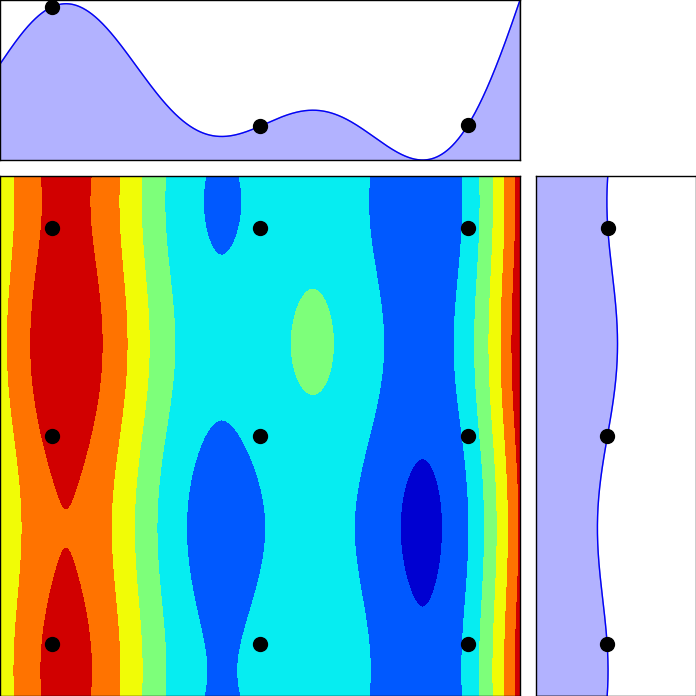
\includegraphics[width=7.2cm]{img_hyperopt/rs_grid}}
	\end{minipage}
	\begin{minipage}[b]{.49\linewidth}
		\centering
		\centerline{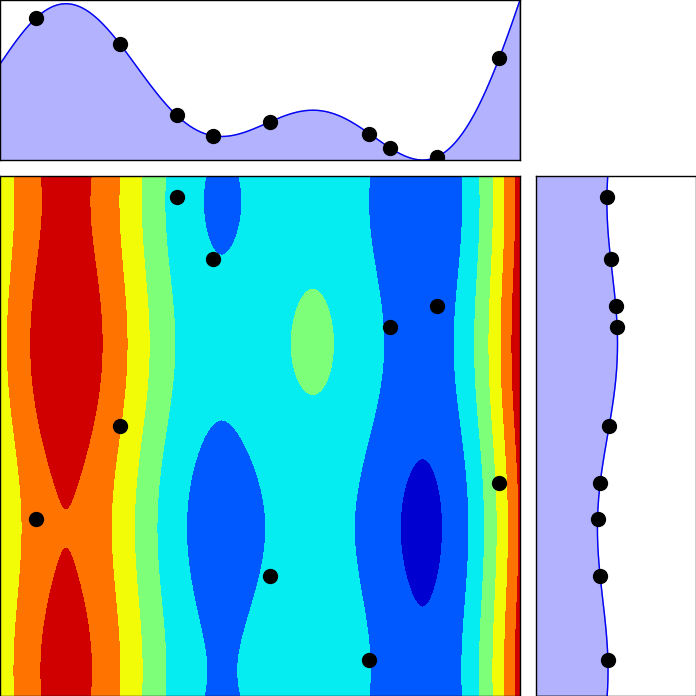
\includegraphics[width=7.2cm]{img_hyperopt/rs_random}}
	\end{minipage}
	\caption{Loss function for a two dimensional space. (Left) Grid search. (Right) Random search. At equal number of tried combinations, random search finds a better solution.}
	\label{fig:rs}
\end{figure}

==Can we do better than random search? Instead of picking combinations randomly from a uniform distribution, we could model the loss directly from the hyper-parameters, then pick the most promising configurations from this model. This is the idea behind Bayesian optimization, which we present in details in Section~\ref{sec:bo}.

==The task of building neural networks is well suited to the use of evolutionary algorithms. Networks can be split and combined in many ways due to their graph structure. It can be done at the layer level or even the unit level. Historically, NEAT~\cite{stanley2002EC} was the most efficient algorithm of this kind. More recent approaches such as~\cite{real2017ICML} or~\cite{miikkulainen2017} are able to explore extremely diverse and atypical network structures, while giving state-of-the-art results. They do require however a huge amount of computation.


As a black-box optimisation problem: random search, bayesian optimisation

Random Search~\textcite{bergstra2012JMLR}

GP + Tree of Parzen Estimator~\textcite{bergstra2011NIPS}

CMA-ES

%%%%%%%%%%%%%%%%%%%%%%%%%%%%%%%%%%
\subsection{As Meta-learning}

==Recently, reinforcement learning methods have been considered for this task~\cite{baker2017ICLR}~\cite{zoph2017ICLR}. A neural network called the controller is trained to build other neural networks, extremely efficient for a given task. It offers the possibility of transfer learning by reusing the controller on tasks similar to the initial one. The difficulty is in training the controller, which requires to build and train thousands of networks. 

==One major advantage of the last two approaches is the ability to use conditional hyper-parameters, i.e. hyper-parameters that must be chosen only if another hyper-parameter was chosen at a particular value. Bayesian Optimization one the one hand and Hyperband on the other hand have no simple way to integrate such hyper-parameters.

As a meta-learning problem: learning to learn, architecture learning

Large scale evolution

%%%%%%%%%%%%%%%%%%%%%%%%%%%%%%%%%%
\subsection{Other approaches}

==In the context of deep learning, the problem can be seen as a multi-armed bandit. The idea is to evaluate the models as soon as possible and discard the unpromising ones without wasting more time training them. The time gained can then be spent trying more models. Section~\ref{ssec:hyperband} describes an algorithm using this concept.

Bandit: Hyperband~\textcite{li2017ICLR}

Spectral Approach~\textcite{hazan2018ICLR}

Extrapolation of learning curves

%%%%%%%%%%%%%%%%%%%%%%%%%%%%%%%%%%
\subsection{Synthesis}

Can we unify all those approaches in the same framework ?

%%%%%%%%%%%%%%%%%%%%%%%%%%%%%%%%%%%%%%%%%%%%%%%%%%%%%%%%%%%%%%%%%%%%%%%%%%%%%%%%%%%%%%%%%%%%%%%
\section{Bayesian Optimization}
\label{sec:bo}

Bayesian Optimization is a method for optimizing the parameters of a black-box that is costly to evaluate. In deep learning the black-box is a neural network and the parameters are the hyper-parameters of the network. Evaluating it corresponds to training the network and computing the performance on the validation set. A recent and general review of the topic can be found in~\textcite{shahriari2016IEEE} where it is treated as an optimization method, while~\textcite{snoek2012NIPS} review the topic in the context of optimizing the hyper-parameters of machine learning models.

There are two components to Bayesian Optimization. First is a probabilistic model of the loss function, i.e. a function that takes the values of the hyper-parameters as input and estimate the value of the loss the corresponding neural network would have. Our model of choice is Gaussian processes which we present in Section~\ref{ssec:gp}. The second component, called the acquisition function, samples the model of the loss function to select the next set of hyper-parameters to evaluate. Common acquisition functions are presented in Section~\ref{ssec:acqfunc}.

%%%%%%%%%%%%%%%%%%%%%%%%%%%%%%%%%%
\subsection{Gaussian Processes}
\label{ssec:gp}

A Gaussian process is a supervised learning model mainly used for regression problems. It is a distribution over functions, i.e. from a set of data points, the Gaussian process gives us possible functions that fit those points, weighted by their likelihood. The shape and properties of possible functions are defined by a covariance function. When predicting the value of an unseen point, the Gaussian process returns a Normal distribution, with the variance an estimation of the uncertainty of the model at this point. Predicting multiple points will result in a joint Gaussian distribution.

Following the notation of~\textcite{rasmussen2005}, we write the Gaussian process as

\begin{equation}
    \mathrm{y}(\mathrm{x}) \sim \mathcal{GP} \left( m(\mathrm{x}), k(\mathrm{x}, \mathrm{x'}) \right)
\end{equation}

where $m(\mathrm{x})$ is the mean function which we set to $0$ for simplicity (in practice, just remove the mean of the predicted values from your dataset), and $k(\mathrm{x}, \mathrm{x'})$ is the covariance function which specifies the covariance between pair of data points. From this function we can build the covariance matrix of a set $\mathrm{X}$ of $N$ data points as

\begin{equation}
    K(\mathrm{X}, \mathrm{X}) = 
    \begin{pmatrix}
    k(\mathrm{x_1}, \mathrm{x_1}) & k(\mathrm{x_1}, \mathrm{x_2}) & \cdots & k(\mathrm{x_1}, \mathrm{x_N}) \\
    k(\mathrm{x_2}, \mathrm{x_1}) & k(\mathrm{x_2}, \mathrm{x_2}) & \cdots & k(\mathrm{x_2}, \mathrm{x_N}) \\
    \vdots & \vdots & \ddots & \vdots \\
    k(\mathrm{x_N}, \mathrm{x_1}) & k(\mathrm{x_N}, \mathrm{x_2}) & \cdots & k(\mathrm{x_N}, \mathrm{x_N})
    \end{pmatrix}
\end{equation}

This matrix is all we need to draw samples from the distribution. We pick a set $\mathrm{X_*}$ of points, build the covariance matrix $K(\mathrm{X_*}, \mathrm{X_*})$, then generate samples from this Gaussian distribution:

\begin{equation}
    \mathrm{y_*} \sim \mathcal{N} \left( 0, K(\mathrm{X_*}, \mathrm{X_*})\right)
\end{equation}

Some such samples are shown in Figure~\ref{fig:gp_prior}. The covariance function chosen for now is the squared exponential kernel:
\begin{equation}
	k(\mathrm{x}, \mathrm{x'}) = \sigma^2 \exp\left( -\frac{||\mathrm{x} - \mathrm{x'}||_2}{2l^2}\right)
\end{equation}
Other kernels and their properties are discussed later. 

Back to Figure~\ref{fig:gp_prior}, the thick blue line represents the mean of the distribution and the blue area around is the $95 \%$ prediction interval, i.e. all drawn samples will be in this interval with a probability of $95 \%$ (for a Normal distribution this is equal to $1.96 \sigma$). 

%The covariance matrix is a Gram matrix, meaning it is positive semi-definite, i.e. it admits a unique Cholesky decomposition

\begin{figure}[htb]
	\centering
	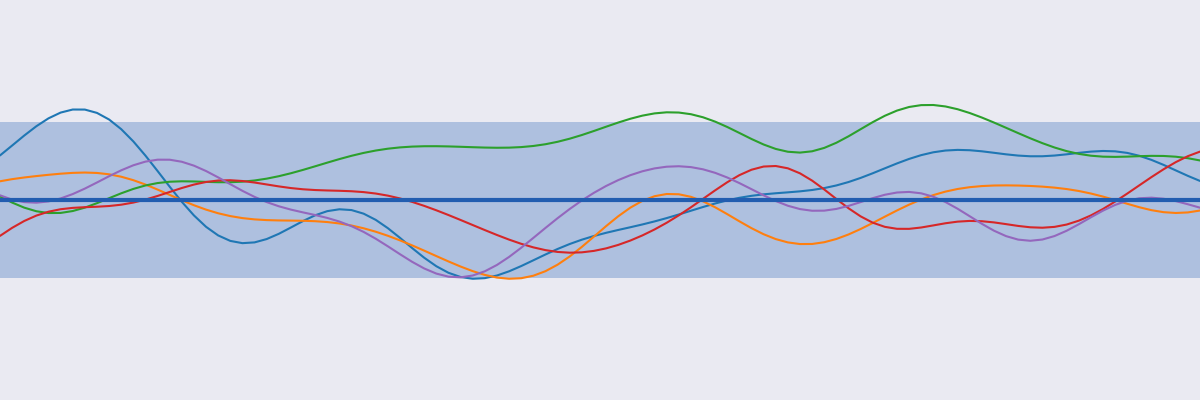
\includegraphics[width=\linewidth]{img_hyperopt/gp_prior.png}
	\caption{Gaussian process prior using a squared exponential kernel. The thin colored lines are samples drawn from the Gaussian process.}
	\label{fig:gp_prior}
\end{figure}

In probabilistic terms, this corresponds to the prior. Given a set of observed points $(\mathrm{X}, \mathrm{y})$ and a set of points we want to predict $(\mathrm{X_*}, \mathrm{y_*})$, the prior corresponds to $p\left( \mathrm{y_*} | \mathrm{X_*}, \theta \right)$ ($\theta$ are the hyper-parameters of the model which we will deal with later). We are interested in the posterior $p\left( \mathrm{y_*} | \mathrm{X_*}, \mathrm{X}, \mathrm{y}, \theta \right)$ i.e. the distribution of the new points conditioned on the points we have already observed. From probability theory we know that the posterior is

\begin{equation}
    p\left( \mathrm{y_*} | \mathrm{X_*}, \mathrm{X}, \mathrm{y}, \theta \right)
    =
    \frac{p\left( \mathrm{y}, \mathrm{y_*} | \mathrm{X}, \mathrm{X_*}, \theta \right)}{p\left( \mathrm{y} | \mathrm{X}, \theta \right)}
\end{equation}

The numerator is called the joint distribution and the denominator is the marginal likelihood. First, we compute the joint distribution

\begin{equation}
    \begin{bmatrix}
    \mathrm{y} \\
    \mathrm{y_*}
    \end{bmatrix}
    \sim
    \mathcal{N} \left( 0, 
    \begin{bmatrix}
    K(\mathrm{X}, \mathrm{X}) & K(\mathrm{X}, \mathrm{X_*}) \\
    K(\mathrm{X_*}, \mathrm{X}) & K(\mathrm{X_*}, \mathrm{X_*})
    \end{bmatrix}
    \right)
\end{equation}

Training a Gaussian process simply means pre-computing $K(\mathrm{X}, \mathrm{X})$, i.e. the covariance between the data points. At inference, we compute the covariance $K(\mathrm{X_*}, \mathrm{X_*})$ between the points we want to predict, and the covariance between the points we have observed and the points we want to predict $K(\mathrm{X}, \mathrm{X_*})$. And since the covariance matrix must be symmetrical, $K(\mathrm{X_*}, \mathrm{X}) = K(\mathrm{X}, \mathrm{X_*})^T$. For notational simplicity we will denote them $K$, $K_*$ or $K_*^T$ and $K_{**}$.

But the joint distribution isn't enough, it will generate functions that do not match the observed data. The posterior is obtained by conditioning the joint distribution to the observations, and because every term involved is a Gaussian distribution, there is a well-known result giving us the following equation

\begin{equation}
    p\left( \mathrm{y_*} | \mathrm{X_*}, \mathrm{X}, \mathrm{y}, \theta \right)
    =
    \mathcal{N} \left( K_* K^{-1} y, 
    K_{**} - K_* K^{-1} K_*^T \right)
\end{equation}

\begin{figure}[htb]
    \centering
    \begin{subfigure}[b]{\textwidth}
        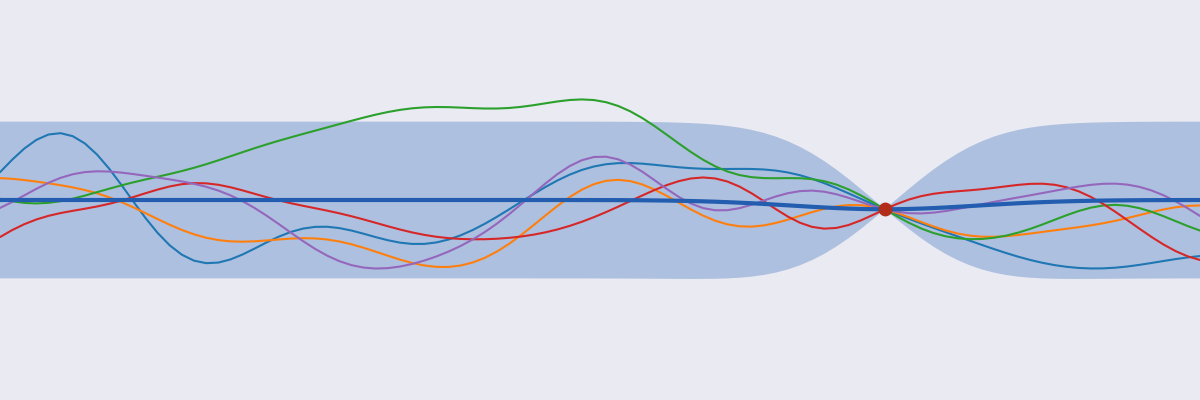
\includegraphics[width=\textwidth]{img_hyperopt/gp_posterior_1_point}
    \end{subfigure}

    \begin{subfigure}[b]{\textwidth}
        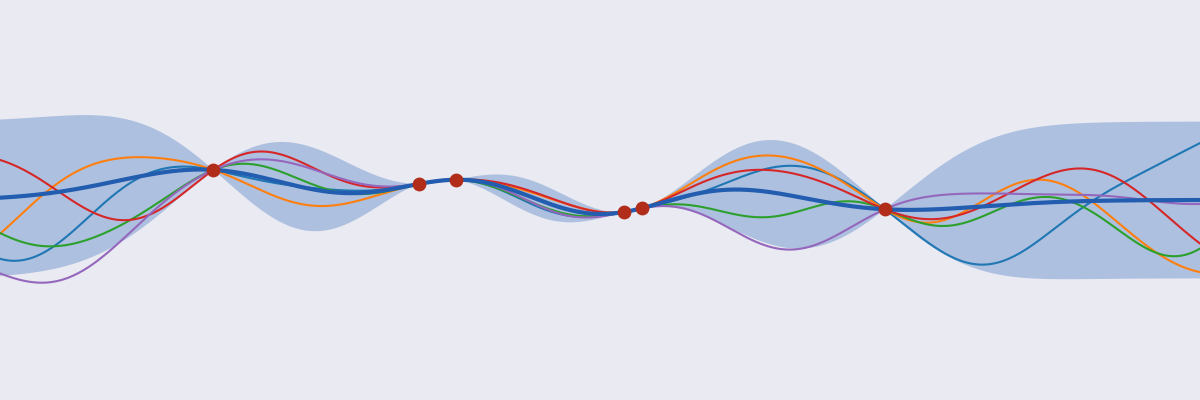
\includegraphics[width=\textwidth]{img_hyperopt/gp_posterior_6_point}
    \end{subfigure}
    \caption{Gaussian process posterior after fitting one point on top, six on the bottom. Notice how all the samples now go through those points and how the variance is lower close to them.}
    \label{fig:gp_posterior}
\end{figure}

Figure~\ref{fig:gp_posterior} shows what samples from this distribution looks like on a one dimensional problem. Each sample must go through every observed point, and the closer the points are, the less freedom the samples have to change. We also observe that outside of the range of points, the distribution quickly reverts to its prior. This is a property of this kernel, which is ill-suited for extrapolation.

So far we have assumed for simplification that the data is noise-free, however it is important to note that Gaussian processes are particularly well-adapted at dealing with noisy data. See~\textcite{rasmussen2005} for the changes to the equations.

We glossed over the choice of kernel until now. The most common is the one we used so far, the squared exponential kernel
\begin{equation}
	k(\mathrm{x}, \mathrm{x'}) = \sigma^2 \exp\left( -\frac{||\mathrm{x} - \mathrm{x'}||_2}{2l^2}\right)
\end{equation}

This kernel has two hyper-parameters $\theta = \{ \sigma^2 , l \}$. $\sigma^2$ controls the scale of the predicted output and $l$ is a vector of same dimensionality as $\mathrm{x}$ called the characteristic length-scale which measures how much a change along each dimension affects the output. A low value means that a small change in the input results in a big change in the output. 

The samples from this kernel are very smooth, and are in fact infinitely differentiable. This is usually too unrealistic for the process we are trying to model. In the context of Bayesian optimization, a more realistic alternative is the Matérn $5/2$ kernel
\begin{equation}
    k(r) = \sigma^2 \left( 1 + \frac{\sqrt{5}r}{l} + \frac{5r^2}{3l^2} \right) \exp \left( - \frac{\sqrt{5}r}{l}\right)
\end{equation}

where $r = \mathrm{x} - \mathrm{x'}$. The Matérn covariance functions are a class of kernel with two parameters $l$ and $\nu$. $\sigma^2$ and $l$ have the same role as for the squared exponential kernel and $\nu$ is a measure of how smooth the function is. The chosen value of $\nu = 5/2$ means the samples will be twice differentiable. $\nu = 1/2$ results in a very rough function while $\nu \to \infty$ is the squared exponential kernel. $5/2$ is a good compromise between too smooth and too difficult to optimize $\theta$ as many point estimate methods requires twice differentiability (\textcite{snoek2012NIPS}). Figure TODO shows what samples from these kernels look like.

[TODO fig influence of $\nu$]

The kernels presented have the common property of being stationary, i.e they depend only of $\mathrm{x} - \mathrm{x'}$. They are invariant to translation. It's very relevant in the context of hyper-parameter optimization as the kernels make no difference between values of 3 and 2 or 1000 and 999. Depending on the meaning of the hyper-parameters, this is not desirable. The solution is to use a non-stationary kernel, which we discuss in Section~\ref{ssec:nosta}.

Another problem of those kernels is that they have themselves hyper-parameters $\theta$ which needs to be chosen. As said before, $l$ is the characteristic length-scale. By construction of those covariance functions and as shown in~\textcite{neal1996phd}, the inverse of the length-scale determines how relevant an input is. In the context of hyper-parameter optimization, it can help us choose which hyper-parameters to tune carefully. It is therefore very important to select the correct value for $l$. 

There are two ways to learn $\theta$. The first is to maximize the marginal likelihood, which can be derived to  
\begin{equation}
	\log p\left(\mathrm{y} | \mathrm{X}, \theta \right) = - \frac{1}{2} \mathrm{y}^T K^{-1} \mathrm{y} - \frac{1}{2} \log |K| - \frac{n}{2} \log 2 \pi
\end{equation}

The optimization can be done with any off-the-shelf method, eventually with multiple restarts as there are no guarantee of a unique optima. 
%For example, the scikit-learn (\textcite{pedregosa2011sklearn}) implementation uses BFGS with 10 restarts by default.

The other solution is to not learn $\theta$ at all and instead marginalize the hyper-parameters, i.e. at inference compute 
\begin{equation}
    p\left( \mathrm{y_*} | \mathrm{X_*}, \mathrm{X}, \mathrm{y} \right)
    = \int p\left( \mathrm{y_*} | \mathrm{X_*}, \mathrm{X}, \mathrm{y}, \theta \right) p \left( \theta | \mathrm{X}, \mathrm{y} \right) d\theta
\end{equation}

This integral is usually intractable but can be approximated by sampling methods. \textcite{murray2010NIPS} use slice sampling, \textcite{garbuno2016CSDA} use asymptotically independent Markov sampling and \textcite{titsias2011} review different Monte Carlo methods used for this problem.

For a more extensive treatment on Gaussian Processes, see~\textcite{rasmussen2005}.

%%%%%%%%%%%%%%%%%%%%%%%%%%%%%%%%%%
\subsection{Acquisition Functions}
\label{ssec:acqfunc}

TODO:
\begin{itemize}
    \item Figure PI vs EI
    \item Should I talk about other functions, even if we didn't use them ? (Upper Confidence Bound, Thompson Sampling, Entropy-search Portfolio)
\end{itemize}

In the context of Bayesian optimization, the Gaussian process gives us for each set of hyper-parameters an estimation of the performance of the corresponding model and the uncertainty of the Gaussian process in its estimation. But we don't have a way to decide which model is the most interesting to train. Do we pick a model that will be slightly better than our best current model, i.e. where the Gaussian process gives low uncertainty, or do we pick a model with high uncertainty but which could have terrible performance ? There is an exploration/exploitation trade-off. It is the role of the acquisition function to determine which model to train.

One acquisition function is the Probability of Improvement (\textcite{kushner1964}). It chooses the model which has the highest probability of having better results than a target, which is usually picked to be the loss of the current best model. The PI is defined as such:
\begin{equation}
    PI(\mathrm{x}) = \Phi \left( \frac{y_* - \mu(\mathrm{x})}{\sigma(\mathrm{x})}\right)
\end{equation}

where $\Phi$ is the Normal cumulative distribution function, $\mathrm{x}$ represents a given set of hyper-parameters, $y_*$ is the minimum loss found so far, $\mu$ is the mean returned by the Gaussian process and $\sigma$ the variance.

The problem with this function is that it is highly sensitive to choice of target. If picked to be the loss of the best model found so far, it will sample models very close to it, meaning we need to specify how much better we want to be. But that's very inconvenient because we usually have no idea how much better we can get. Should we try to find a model $1 \%$ better ? $5 \%$ ? $25 \%$ And if we pick too big of an improvement, the function will simply select the models with the highest uncertainty.

Instead, we can use the Expected Improvement function (\textcite{schonlau1998}) which build on the Probability of Improvement:
\begin{equation}
	EI(\mathrm{x})  = \sigma (\mathrm{x}) [u\Phi(u)+\phi(u)]
\end{equation}
with
\begin{equation}
	u = \frac{y_* - \mu(\mathrm{x})}{\sigma(\mathrm{x})}
\end{equation}

where $\phi$ is the normal density function. EI is obtained by taking the expectation of the improvement function (\textcite{shahriari2016IEEE}), defined as such:

\begin{equation}
	I(\mathrm{x}) = \left(y_* - \mu(\mathrm{x}) \right) \mathds{1} \left(y_* > \mu(\mathrm{x}) \right)
\end{equation}
This function is equal to $0$ if the predicted mean is less than the best loss found so far (which means that there is no improvement), otherwise it is proportional to the gap between the predicted mean and best loss. 

The Expected Improvement has one big advantage over the Probability of Improvement. The target is always the minimum loss found so far, meaning there is no need to guess a threshold of improvement. 

An extended discussion on the trade-offs between Probability of Improvement and Expected Improvement can be found in~\textcite{jones2001}.

%%%%%%%%%%%%%%%%%%%%%%%%%%%%%%%%%%
\subsection{Tying it together}

TODO:
\begin{itemize}
    \item Figure step-by-step BO
\end{itemize}

Let's resume the situation. We are trying to find the best model in a large family of models in a reasonable amount of time. We have already trained some models and are trying to decide which model to train next. First, we fit a Gaussian process on the models already trained, with the hyper-parameters as the input, and the loss of the corresponding model as the output. We then sample new combinations and have them predicted by the Gaussian process. For each sample, we also compute the Expected Improvement. The next model to train is the one with the highest EI. Once it's trained, we fit again the Gaussian process with the new information, and we repeat the process until we run out of time or we obtain a model good enough for our purposes. Figure~\ref{fig:bo} shows this process on a one-dimensional problem.

\begin{figure}[htb]
	\centering
	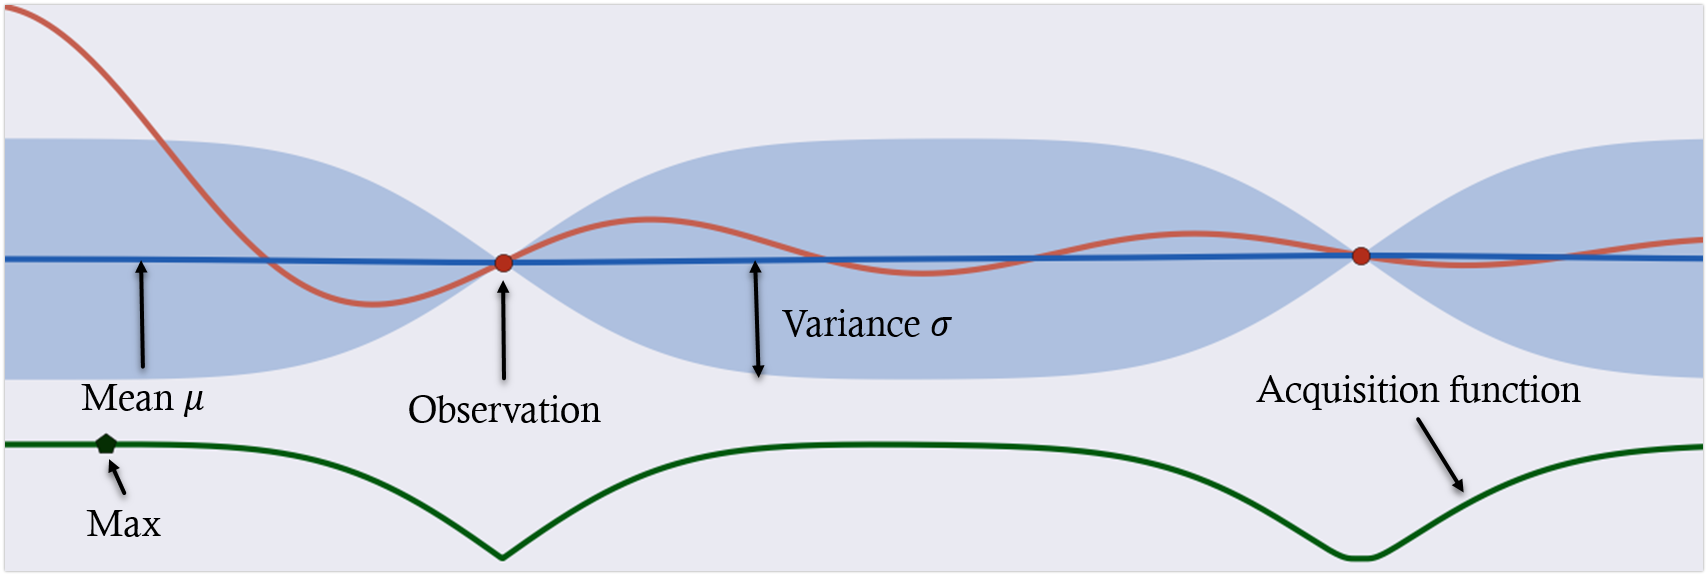
\includegraphics[width=\linewidth]{img_hyperopt/bo.png}
	\caption{Bayesian Optimization on a one dimensional function. The orange curve is the true loss function, the blue one is the prediction of the Gaussian process. The green curve is the acquisition function. The next evaluation will be at the maximum of the green curve.}
	\label{fig:bo}
\end{figure}

Some questions remain. How to pick the first model ? Select a random configuration of hyper-parameters from the hyper-parameter space. What loss should the Gaussian process predict ? Ideally, the loss of the model on the validation set. Otherwise the loss on the training set works fine. How to sample configurations ? Uniformly from the hyper-parameter space. How many configurations should be sampled before selecting a model to train ? As many as reasonably possible. The step of selecting a model should be much faster than training it, and most of the cost of Bayesian optimization should be in the inversion of the Gram matrix (see Section~\ref{ssec:practical} for details).

%Hyperopt~\textcite{bergstra2013ICML}

%Practical~\textcite{snoek2012NIPS}

%%%%%%%%%%%%%%%%%%%%%%%%%%%%%%%%%%
\subsection{Practical Challenges}
\label{ssec:practical}

%==One important aspect of this method is that the training time of the model is a dimension of the hyper-parameter space. This means that the method is free to choose how long to train each model. In practice we found that it prefers longer training time, even though it looks like a lower training time is enough to get a good estimate of the worth of the model and would allow the evaluation of more models. This is a flaw of the method, which lacks an explicit notion of budget and a way to best exploit it.

\subsubsection{Conditional spaces}

TODO
\begin{itemize}
    \item Describe cylindrical embeddings
    \item Describe tree of Parzen estimator
\end{itemize}

The version of Bayesian optimization we presented deals efficiently with both discrete and continuous hyper-parameters. But what about conditional hyper-parameters ? For example, some hyper-parameter could be specific to a particular layer and one hyper-parameter could control the number of layers. But then, what happens to the hyper-parameters of a non-existent layer ? With a Gaussian process, we need to give them a value and it means there will be many configurations that corresponds to the same model. In practice, we can ignore those cases, and the Gaussian process will eventually give a low uncertainty in those regions and pick models elsewhere. But this is extremely wasteful as we will retrain the same model many times before this happens ! 

One solution is to use a specialized kernel called a cylindrical kernel (\textcite{swersky2013},~\textcite{oh2018}).

Another solution is to not use a Gaussian process at all. It has been our model of choice so far but other alternatives exist. One such alternative is tree-structured Parzen estimator (\textcite{bergstra2011NIPS}).

\subsubsection{Parallelization}

Open problem using GP

See combination with Hyperband for a potential solution

\subsubsection{Non-stationarity}
\label{ssec:nosta}

Input Warping~\textcite{snoek2014ICML}

\subsubsection{Scaling}

Doesn't work well in high-dimension or with thousands of data points

Conditional neural processes ?

%%%%%%%%%%%%%%%%%%%%%%%%%%%%%%%%%%
\subsection{Contribution: Incremental Cholesky decomposition}

TODO:
\begin{itemize}
    \item Rewrite the explanation
    \item Should I put the full proof of the results here ? In an appendix ?  
\end{itemize}

One of the big timesink of GP: computing the Cholesky decomposition. But in BO, the Gram matrix between calls is mostly the same, just with new rows. So we can store the decomposition and just update it.

==An important property of Gaussian processes is that the Gram matrix $K$ always has a unique Cholesky decomposition ($K$ is definite positive). This property is used in practice for the prediction of the mean and variance because it is necessary to invert $K$, and it is much more efficient to invert the Cholesky decomposition $L$.

==We use here the structure of the Gram matrix and a property of Bayesian optimization in order to reduce significantly the cost of the decomposition. The property is the following: at every call of the Gaussian process, our training set contains $n$ points from before and $k$ new points. By keeping the order of the points, the new Gram matrix is always structured as follows:
\begin{equation}
	K_{(n+k,n+k)} = 
    \begin{pmatrix}
    K_{(n,n)} & K_{(k,n)}^T \\
    K_{(k,n)} & K_{(k,k)}
  \end{pmatrix}
\end{equation}

==Moreover,
\begin{equation}
	 K_{(n,n)} = L_{(n)} L_{(n)}^T
\end{equation}
is already known. The question is then: can we compute $L_{(n+k)}$ from $L_{(n)}$ and the $k$ new points? The answer is positive, and after a bit of arithmetics omitted here, we get this:
\begin{equation}
  L_{(n+k)} = 
  \begin{pmatrix}
    L_{(n)} & 0 \\
    K_{(k,n)} (L_{(n)}^T)^{-1} & L_{(k)}
  \end{pmatrix}
\end{equation}

==It is also possible to get a formula for $ L_{(n+k)}^{-1}$:
\begin{equation}
  L_{(n+k)}^{-1} =
  \begin{pmatrix}
    L_{(n)}^{-1} & 0 \\
    - L_{(k)}^{-1} K_{(k,n)} (L_{(n)}^T)^{-1} L_{(n)}^{-1} & L_{(k)}^{-1}
  \end{pmatrix}
\end{equation}

==The complexity of the Cholesky decomposition is $O\left(\frac{(n+k)^3}{3}\right)$. In our case, this becomes $O\left(\frac{k^3}{3}\right)$ since it is still necessary to compute the decomposition of the $k$ new points.

%%%%%%%%%%%%%%%%%%%%%%%%%%%%%%%%%%%%%%%%%%%%%%%%%%%%%%%%%%%%%%%%%%%%%%%%%%%%%%%%%%%%%%%%%%%%%%%
\section{Application: Classification of MRI Field-of-View}

This section describes and extend work that was presented at ISBI 2017.

%==starting from a baseline network (Section~\ref{ssec:baseline}), we present an automatic strategy to find better architectures given our clinical context. We constrain our search to a space of networks represented by a specific parametrization (Section~\ref{ssec:param}) that includes enough diversity and, at the same time, promising models (including AlexNet-like, VGG-like). Inspired by the work in~\cite{jones_taxonomy_2001}, we devise an automatic optimization process (Section~\ref{ssec:search}) to produce an ensemble of successful models (Section~\ref{ssec:ensemble}). The interest and efficiency of this strategy are demonstrated on our application in Section~\ref{sec:results}.

%%%%%%%%%%%%%%%%%%%%%%%%%%%%%%%%%%
\subsection{Dataset and Problem Description}

TODO:
\begin{itemize}
    \item Update table
    \item Pick better images from the dataset
\end{itemize}

\begin{figure}
        \begin{subfigure}[b]{0.25\textwidth}
                \centering
                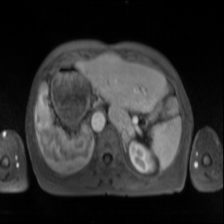
\includegraphics[width=.95\linewidth]{img_hyperopt/abdo_1}
        \end{subfigure}%
        \begin{subfigure}[b]{0.25\textwidth}
                \centering
                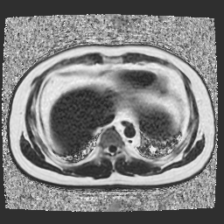
\includegraphics[width=.95\linewidth]{img_hyperopt/abdo_2}
        \end{subfigure}%
        \begin{subfigure}[b]{0.25\textwidth}
                \centering
                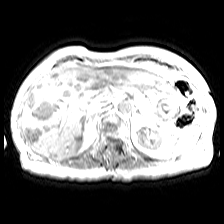
\includegraphics[width=.95\linewidth]{img_hyperopt/abdo_3}
        \end{subfigure}%
        \begin{subfigure}[b]{0.25\textwidth}
                \centering
                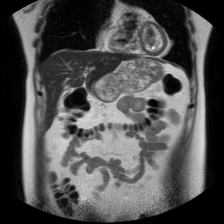
\includegraphics[width=.95\linewidth]{img_hyperopt/abdo_4}
        \end{subfigure}
        \caption{Examples of abdomen in our dataset showing the great variety of protocols}
        \label{fig:abdomens}
\end{figure}

Given an MRI volume we would like to know which anatomical region are contained in it and their position in the volume. Since MRI data is acquired in a slice by slice approach, we reduce the problem to a two dimension classification task (into head, chest, abdomen, pelvis, legs and spine).

\begin{table}
	\centering
	\begin{tabular}{ | l | c | r | }
		\hline
		Body Part & \# Volumes & \# Slices \\ \hline
		Head & 301 & 9032 \\
		Abdomen & 282 & 11532 \\
		Pelvis & 225 & 8854 \\
		Spine & 386 & 7732 \\
		\hline
	\end{tabular}
	\caption{Content of the dataset.}
	\label{table:dataset}
\end{table}
% FIXME: pour la version finale: ajouter min/mean/max slices par volumes

The dataset consists of MRI images coming from a variety of hospitals and machines across the world (such as the \textit{Centre Hospitalier Lyon-Sud, France} or \textit{ Johns Hopkins University, USA}). As a consequence our images display a large variety of protocols (see Figure [TODO]) as well as resolution and number of slices per volume. Table~\ref{table:dataset} sums up the content of our dataset.

The dataset is splitted in a training set for the optimization of the weights $W$, a validation set for model selection (optimization w.r.t hyper-parameters) and a test set for model evaluation (resp. $50 \%$, $25 \%$, $25 \%$). The separation is done volume-wise to take into account intra-subject slices correlations. Volumes containing multiple classes are split by anatomical regions and can end up in different sets. This raises the difficulty of the task since, in case of overfitting, predictions will be wrong at validation or testing phases.
% FIXME: pour la version finale: combien de volumes multi-classes ?
We also stratified classes across sets, giving us a proportion of slices per class close to the proportion of volumes per class.

Finally, each slice is subject to a unique step of preprocessing: it is resized to $128 \times 128$ pixels, a good trade-off between time constraints and quality of information.

Data augmentation consists in generating 80 000 images per epoch, which is 4 times as many images as the training set. The augmentation is done by applying translations, shearing and rotations, zooming, and adding noise.

%%%%%%%%%%%%%%%%%%%%%%%%%%%%%%%%%%
\subsection{Baseline Results}

TODO:
\begin{itemize}
    \item Baseline figure
    \item Performance of the baseline ?
\end{itemize}

Starting from a standard VGG architecture (from~\textcite{simonyan2014}), we modified it manually until settling on the following model: divided in 5 blocks, each comprising a convolution layer of 64 filters of size $3\times 3$, followed by a rectified linear unit (ReLu) and a max-pooling layer. The network ends with 2 fully-connected layers (resp. 4096 and 1024 units) interleaved with ReLU activations and terminated with a softmax decision layer. This network was trained by minimizing the categorical cross-entropy loss weighted by class frequency (denoted $L$ in the rest of this paper), using stochastic gradient descent (SGD) with Nesterov momentum ($m = 0.9$) and decay ($d = 10^{-6}$) .

%%%%%%%%%%%%%%%%%%%%%%%%%%%%%%%%%%
\subsection{Hyper-parameter Optimization}

TODO:
\begin{itemize}
    \item Figure network hyper-params
    \item Details on the optim: number of models tested, ...
    \item Redo results
\end{itemize}

By relaxing some structural parts of our baseline architecture we define a large family of models. This parametric family has the following structure (see Figure \ref{fig:par_archi}): (1) a convolution block comprising $b$ sections, each including $c$ convolution layers of $2^r$ filters of size $s \times s$ interleaved with ReLU activations and terminated by a max-pooling layer, (2) the fully-connected layers as in our baseline architecture, and (3) a final softmax decision layer. 

Changes within this parametric space of models may drastically transform the optimization landscape, requiring to adjust training setting accordingly (in our case: learning rate, batch size and number of epochs, all other settings remaining identical). Moreover, using or not data augmentation is also considered, since more complex models require an increased amount of information.
These architecture parameters and training settings form a collection of model hyper-parameters. Their respective ranges, detailed in Table~\ref{table:hyper}, were defined so as to fulfill memory (less than 12GB) and time constraints (training should last less than one day).

\begin{table}
	\centering
	\begin{tabular}{ | l | c | r | }
		\hline
		Name & Range & Baseline \\ \hline
		\# blocks & $b \in [1 ; 5]$ & $5$ \\
		\# conv. layers per block & $c \in [1 ; 7]$ & $1$ \\
		\# filters per conv. layer & $2^{r}, r \in [2, 7]$ & $64$ \\
		Size of the filters & $ s \in \{3 ; 5\}$ & $3$ \\
		Learning Rate & $10^{l}, l \in [-7 ; 0]$ & $0.001$ \\
		Batch Size & $2^{a}, a \in [2 ; 8]$ & 8 \\
		\# epochs & $10e, e \in [1 ; 10]$ & $70$ \\
        Data augmentation & $g \in \{\text{Yes}, \text{No}\}$ & Yes \\
		\hline
	\end{tabular}
	\caption{Description of the hyper-parameter space, with their range and and the baseline value.}
	\label{table:hyper}
\end{table}

We explored this hyper-parameter space with Bayesian optimization, as described in Section~\ref{sec:bo}. [TODO specific conditions]

At the end, our optimization process yields a collection of models ranked by their performance. The quality of this assessment is naturally limited since the size of the validation set used in this respect cannot encompass the diversity of clinical reality. Cross-validation could be used to get a better estimator of the performance, but we cannot practically afford its costs. Nevertheless, best models present very similar error rates and, at the same time, a good diversity of architectures (see Figure \ref{fig:best_models_archi}) that can be leveraged. We selected the top-ten models and built a robust classifier by averaging their predictions (other combinations could be used as well).

==Figure \ref{fig:best_models_archi} shows the architecture of some of the best models chosen for our ensemble. Despite the first two differing only in the number of blocks, others display variations across all hyper-parameters except data augmentation, which is always turned on. The learning rate is in a small range, either $0.0001$ or $0.001$, and the batch size is small (less than 16). Those networks tend to be deep (min. 8 convolutional layers) and the other hyper-parameters use a wide range of values.

==In terms of accuracy, the ensemble is slightly better than the best model alone, however the ensemble benefits from a reduced bias.

==Figure~\ref{fig:conf} shows the confusion matrices on the test set of the baseline and the ensemble of the 10 best models, demonstrating a substantial improvement on the classification of all anatomical regions. Most of the errors come from pelvis and abdomen, which was expected since the delimitation between those regions is ill-defined. In both cases pelvis is the class with the highest error.

==For the volume classification, the choice of class is done by a majority vote on all slices of the volume. This gives us a higher accuracy. The ensemble misclassifies 444 slices from 71 volumes, but only 7 volumes produce errors. The misclassified slices usually correspond to the first or last one of a volume, containing little information or being nearly part of another anatomical region.

\subsection{Discussion and Conclusion}

TODO
\begin{itemize}
    \item Redo full body figure
\end{itemize}

\begin{figure}[htb]
	\centering
	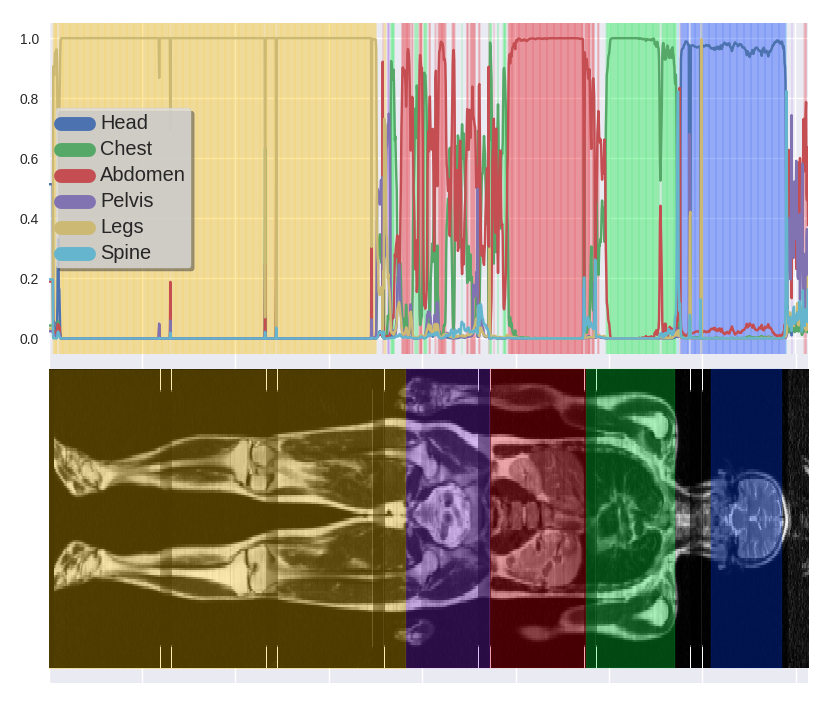
\includegraphics[width=.95\linewidth]{img_hyperopt/full_body_updated}
	\caption{Slice by slice prediction on a full body volume. (Top) Prediction. (Bottom) Ground truth.}
	\label{fig:full_body}
\end{figure}

==As an interesting example, we analyzed a full body volume by classifying each of its slices through our ensemble model. For each slice, the predicted class is the one with a probability higher than 0.7, and if no class meets this criterion, then we do not choose any. As we can see in Figure~\ref{fig:full_body}, the network is doing well at identifying the abdomen and the head. It also identifies correctly the pelvis, with some uncertainty. No class is dominant for most of the legs, however the feet are considered as spine with high probability. It also mistakenly identifies the neck as pelvis.

==Those mistakes could be corrected by using a more complex decision criterion than a simple probability cutoff. We also expect that adding more anatomical regions to our dataset will allow for a better localization of the present regions.

==To the problem of finding more accurate networks than handcrafted ones, we have answered with two viable strategies. Random search is as easy to implement as grid search and quickly improves on the baseline, which makes it perfect for time-constrained situations. Without this constraint and at a higher cost in implementation, an adaptive search based on Gaussian Processes explores a range of highly accurate models suited for ensembling.% The search can be started immediately in adaptive mode, as the GP will have high uncertainty everywhere, resulting in an almost uniform distribution.

==For the hyper-parameters where there is a ``correct" answer, such as the learning rate (0.001) and the presence of data augmentation, the guided search quickly converges and most models inherit their values. We should remove them on further analysis and instead explore a wider range of architectures by adding hyper-parameters controlling the fully-connected layers, such as the number of units, the number of layers, adding new types of layers such as dropout and batch normalization placed across the network or even explore other learning method such as RMSProp or Adadelta. 

==One limitation of the current system is that some hyper-parameters depend on the value of others. For example we are unable to choose a different number of filters per layer as the number of layers is not fixed. We also limited the range of some hyper-parameters such as the filter size so as to have networks that would fit in memory and be trained in a reasonable amount of time. Only a subset of values combinations would cause a failure. Further work could incorporate constraints on time and memory either by precise estimations when possible or by measures during training to produce estimations with a GP. 

==Results on volume classification were very satisfactory. Since it is done at slice level, we have obtained a decent localization tool which shows the robustness of our ensemble. Further work will focus on adding more anatomical regions, which might require splitting slices in patches to identify smaller regions such as organs.

%%%%%%%%%%%%%%%%%%%%%%%%%%%%%%%%%%%%%%%%%%%%%%%%%%%%%%%%%%%%%%%%%%%%%%%%%%%%%%%%%%%%%%%%%%%%%%%
\section{Contribution: Combining Bayesian Optimization and Hyperband}

CAp

%%%%%%%%%%%%%%%%%%%%%%%%%%%%%%%%%%
\subsection{Hyperband}
\label{ssec:hyperband}

==A property of neural networks is that their training is iterative, usually some variant of gradient descent. A consequence is that it is possible to interrupt training any time, evaluate the network, then resume training. This is the property Hyperband~\cite{li2017ICLR} takes advantage of.

==The principle is simple: pick randomly a group of configurations from a uniform distribution, train the corresponding networks partially, evaluate them, resume training of the most performing ones, and so on until a handful of them have been trained to completion. Then pick a new group and repeat the cycle until exhaustion of the available resources.

==But a problem appears: at which point in the training can we start evaluating the models? Too soon and they will not have started to converge, making the evaluation meaningless, too late and we have wasted precious resource training under-performing models. Moreover, we do not know how to find that point and it changes between tasks. Hyperband's answer is to divide a cycle into brackets. Each bracket has the same quantity of resource at its disposal. The difference between brackets is the point at which they start evaluating the models. The first bracket will start evaluating and discarding models very early, allowing it to try a bigger number of configurations, while the last bracket will try only a small number of configurations but will train them until the end.

==The algorithm is controlled by two hyper-parameters: the maximal quantity of resources $R$ that can be allocated to a given model, and the proportion of configurations $\eta$ kept at each evaluation. We chose $R = 27$ minutes and $\eta = 3$, which means that we keep $1/3$ of models at each evaluation.

%%%%%%%%%%%%%%%%%%%%%%%%%%%%%%%%%%
\subsection{Combining the methods}

\begin{figure}[htb]
	\centering
	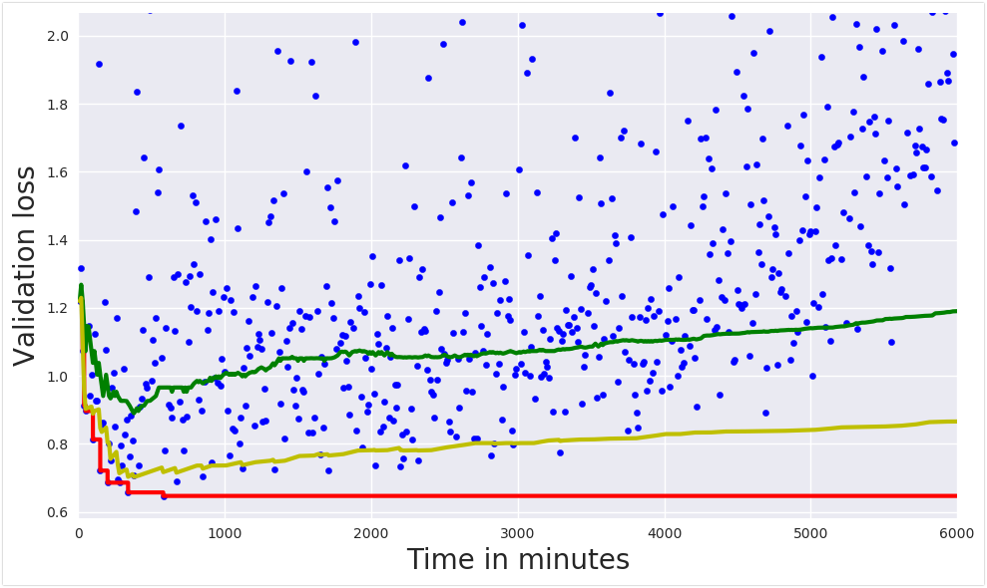
\includegraphics[width=.95\linewidth]{img_hyperopt/bo_acc_time.png}
	\label{fig:bo_acc_time}
\end{figure}

\begin{figure}[htb]
	\centering
	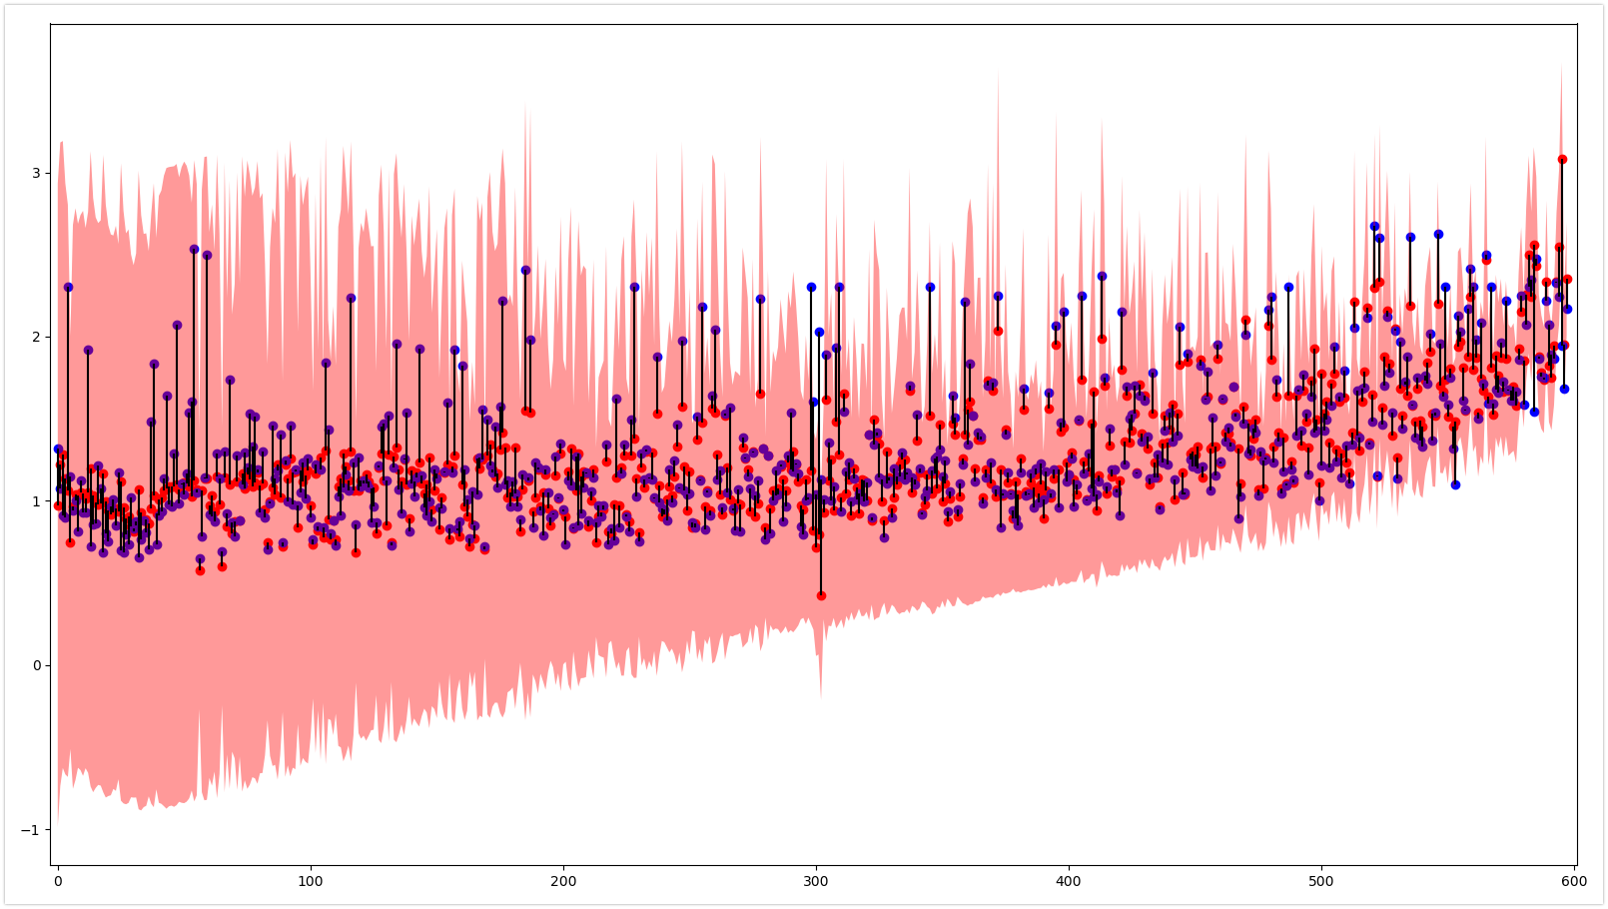
\includegraphics[width=.95\linewidth]{img_hyperopt/bo_error_time.png}
	\label{fig:bo_error_time}
\end{figure}

%%%%%%%%%%%%%%%%%%%%%%%%%%%%%%%%%%
\subsection{Experiments on CIFAR-10}

%%%%%%%%%%%%%%%%%%%%%%%%%%%%%%%%%%%%%%%%%%%%%%%%%%%%%%%%%%%%%%%%%%%%%%%%%%%%%%%%%%%%%%%%%%%%%%%
\section{Conclusion}

When to optimize and with which method ?
